\chapter{Gestik forslag til de valgte funktioner}
\label{app:GestikForslagFunktioner}
%
\section{Forslag til pause og start}
\label{app:ForslagPauseOgStart}
%
Følgende fremgår de syv forskellige forslag til semaforiske gestikker, der kan knyttes til pause og start.
%
\begin{figure}[H]
	\centering
	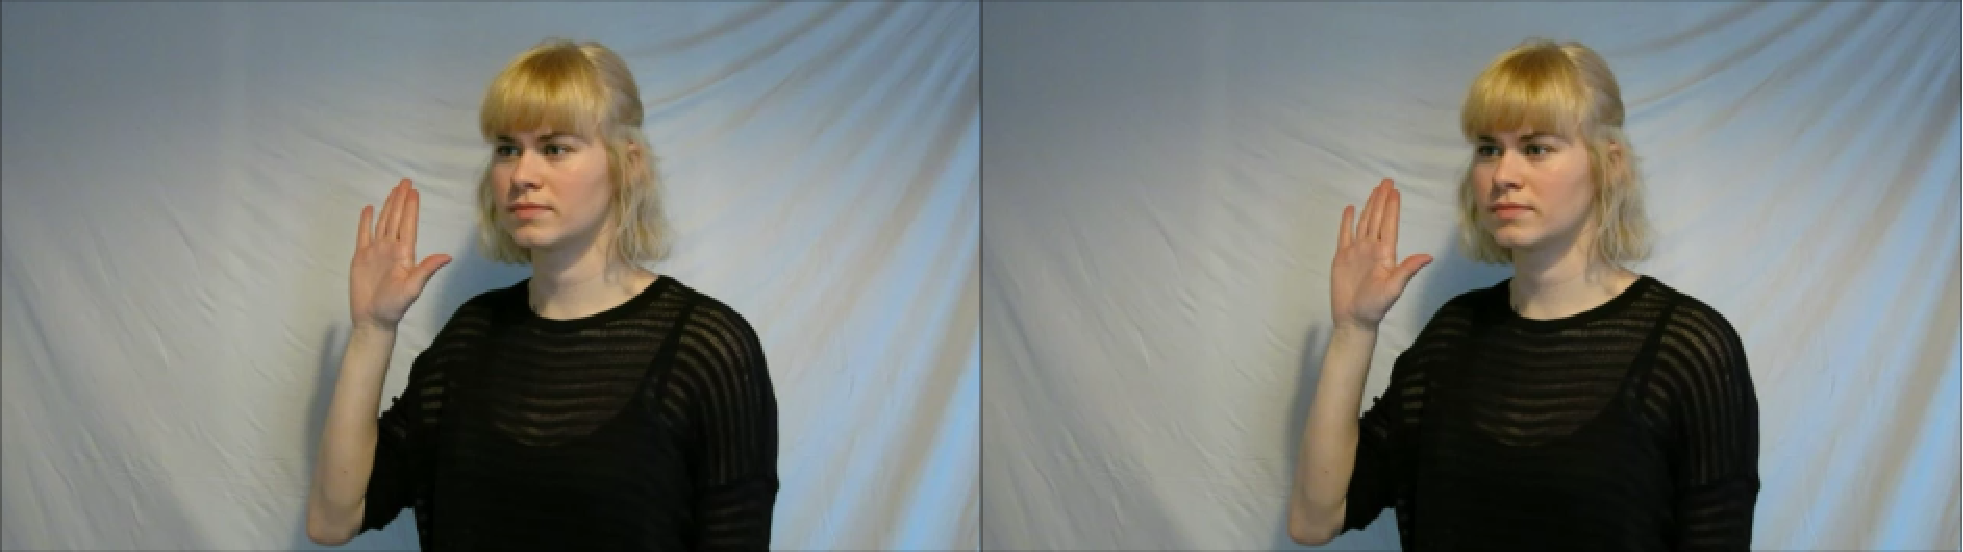
\includegraphics[resolution=300,width=0.9\textwidth]{Test1/Gestik-par/Gestik1_Pause}
	\caption{Illustration af gestik-par 1; stop-tegn til henholdsvis pause og start.}
	\label{fig:GestikPar1PauseApp}
\end{figure}
\noindent
%
%
\begin{figure}[H]
	\centering
	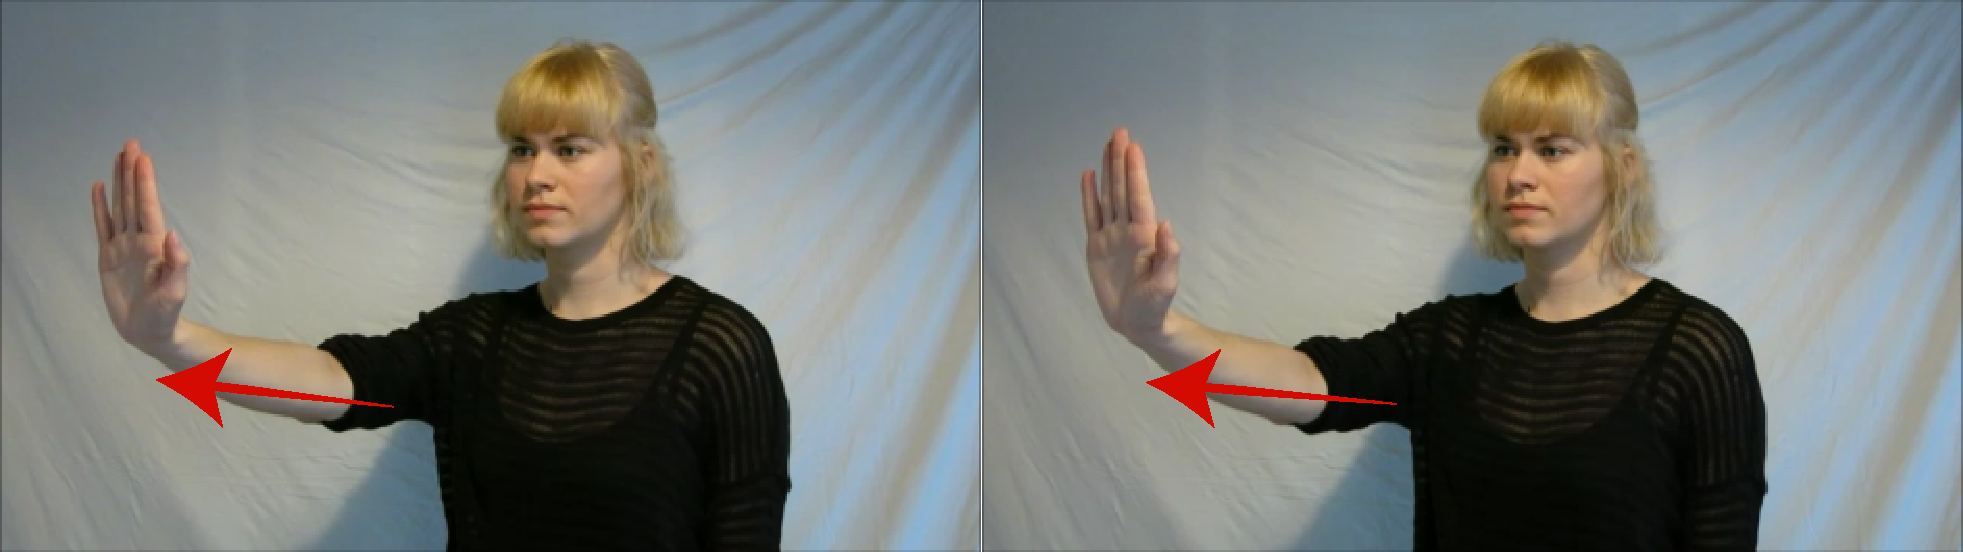
\includegraphics[resolution=300,width=0.9\textwidth]{Test1/Gestik-par/Gestik2_Pause}
	\caption{Illustration af gestik-par 2; dynamisk vertikal hånd, der starter ved brystet og ender i en udstrakt horisontal arm.}
	\label{fig:GestikPar2PauseApp}
\end{figure}
\noindent
%
%
\begin{figure}[H]
	\centering
	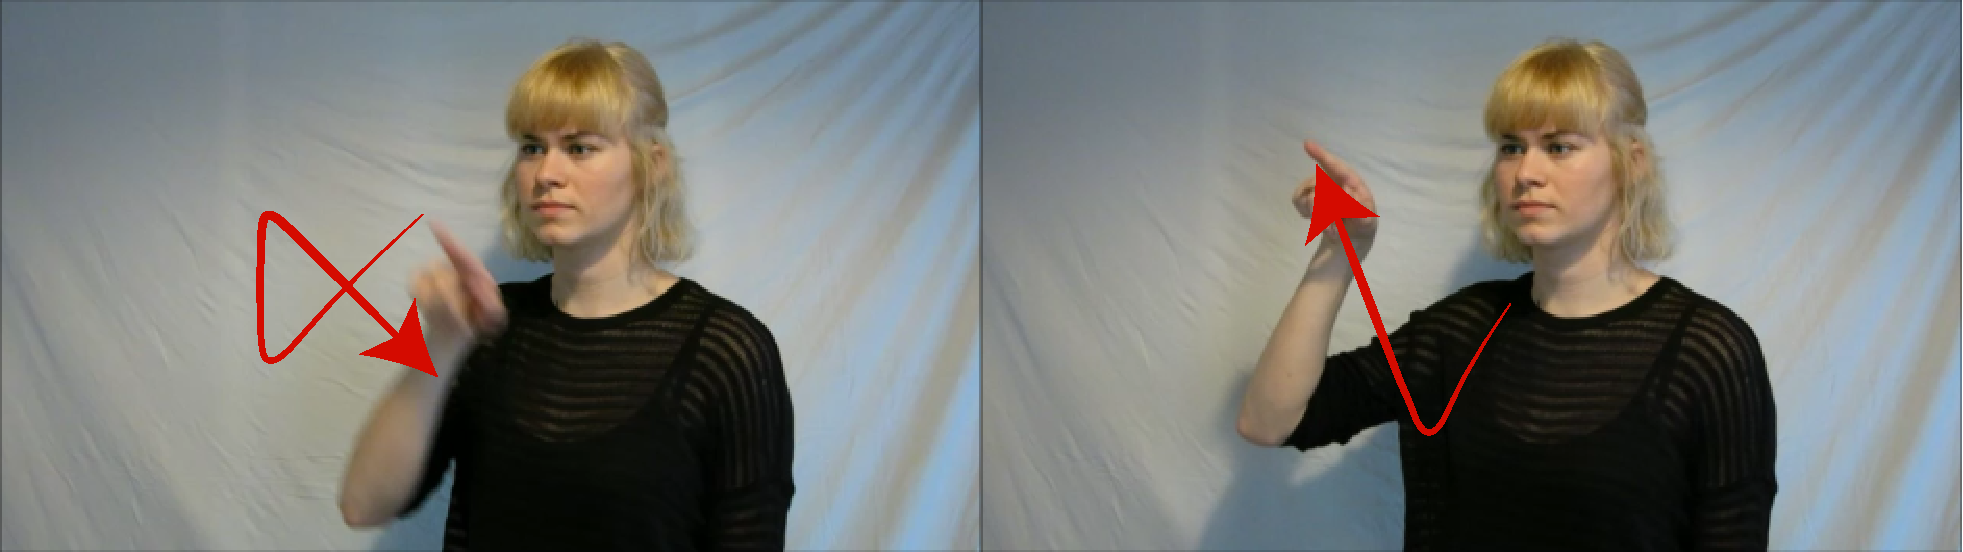
\includegraphics[resolution=300,width=0.9\textwidth]{Test1/Gestik-par/Gestik3_Pause}
	\caption{Illustration af gestik-par 3; kryds til pause og flueben til start.}
	\label{fig:GestikPar3PauseApp}
\end{figure}
\noindent
%
%
\begin{figure}[H]
	\centering
	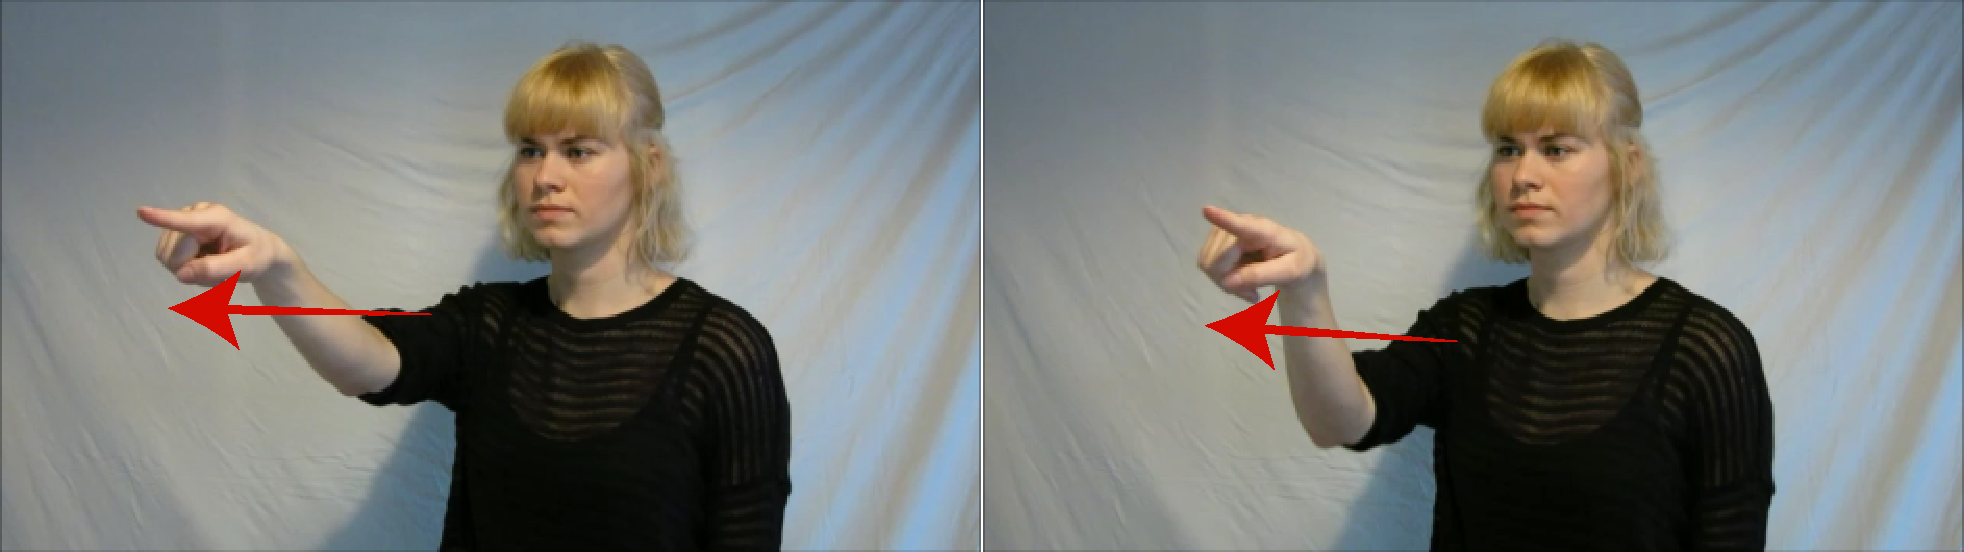
\includegraphics[resolution=300,width=0.9\textwidth]{Test1/Gestik-par/Gestik4_Pause}
	\caption{Illustration af gestik-par 4; pegefingeren peger og trykker i luften hen mod musikanlægget for henholdvis pause og start.}
	\label{fig:GestikPar4PauseApp}
\end{figure}
\noindent
%
%
\begin{figure}[H]
	\centering
	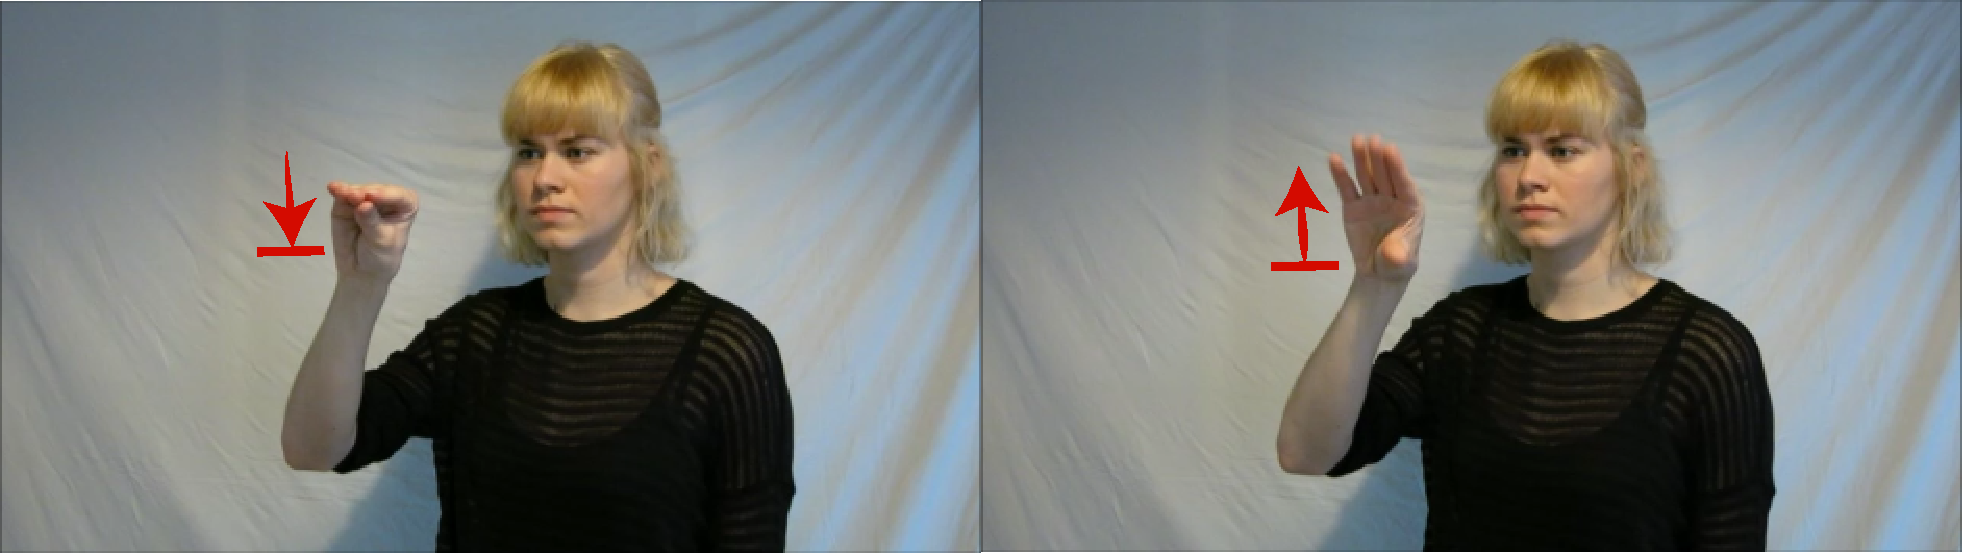
\includegraphics[resolution=300,width=0.9\textwidth]{Test1/Gestik-par/Gestik5_Pause}
	\caption{Illustration af gestik-par 5; krokodillenæb til henholdvis pause og start.}
	\label{fig:GestikPar5PauseApp}
\end{figure}
\noindent
%
%
\begin{figure}[H]
	\centering
	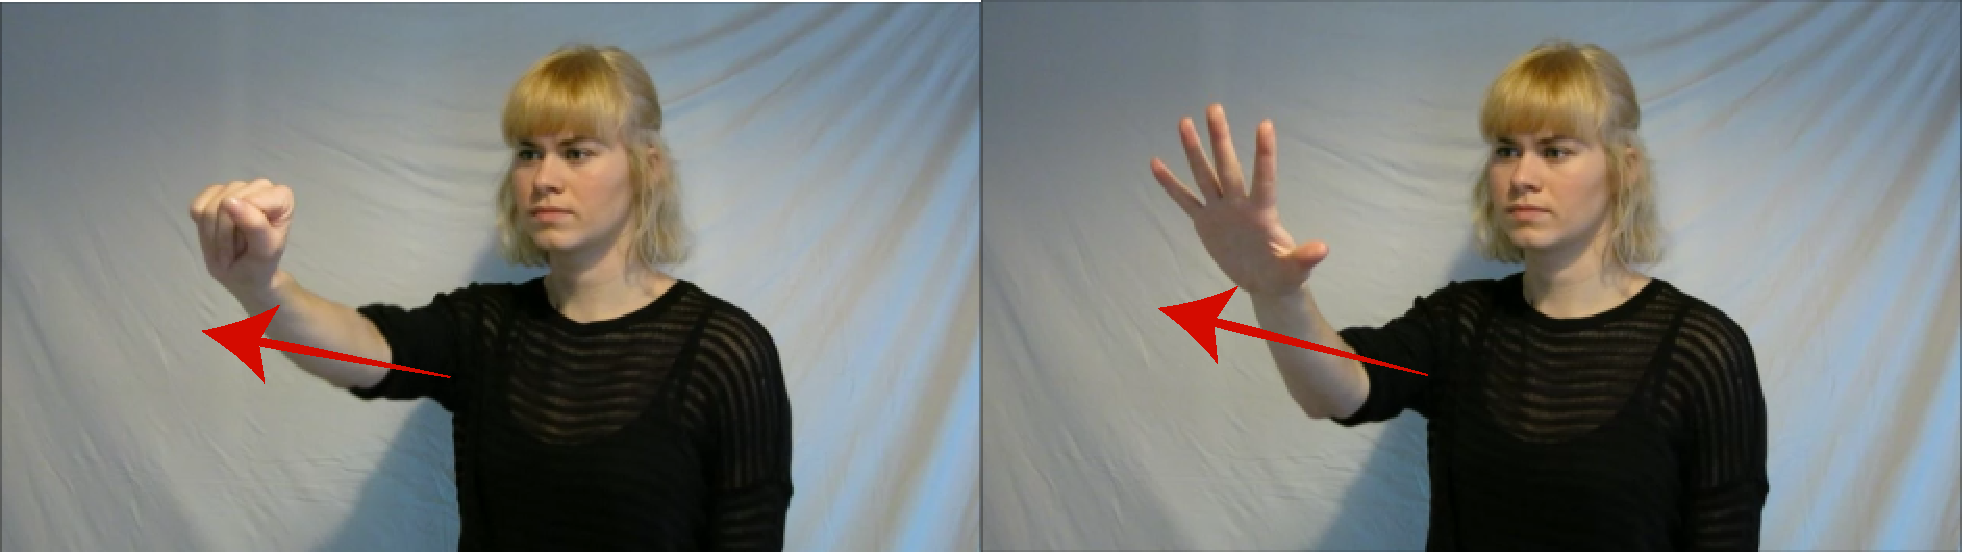
\includegraphics[resolution=300,width=0.9\textwidth]{Test1/Gestik-par/Gestik6_Pause}
	\caption{Illustration af gestik-par 6; hånden lukker sammen i den dynamisk, horisontal bevægelse fremad til pause og hånden åbner i den dynamisk, horisontal bevægelse fremad til start.}
	\label{fig:GestikPar6PauseApp}
\end{figure}
\noindent
%
%
\begin{figure}[H]
	\centering
	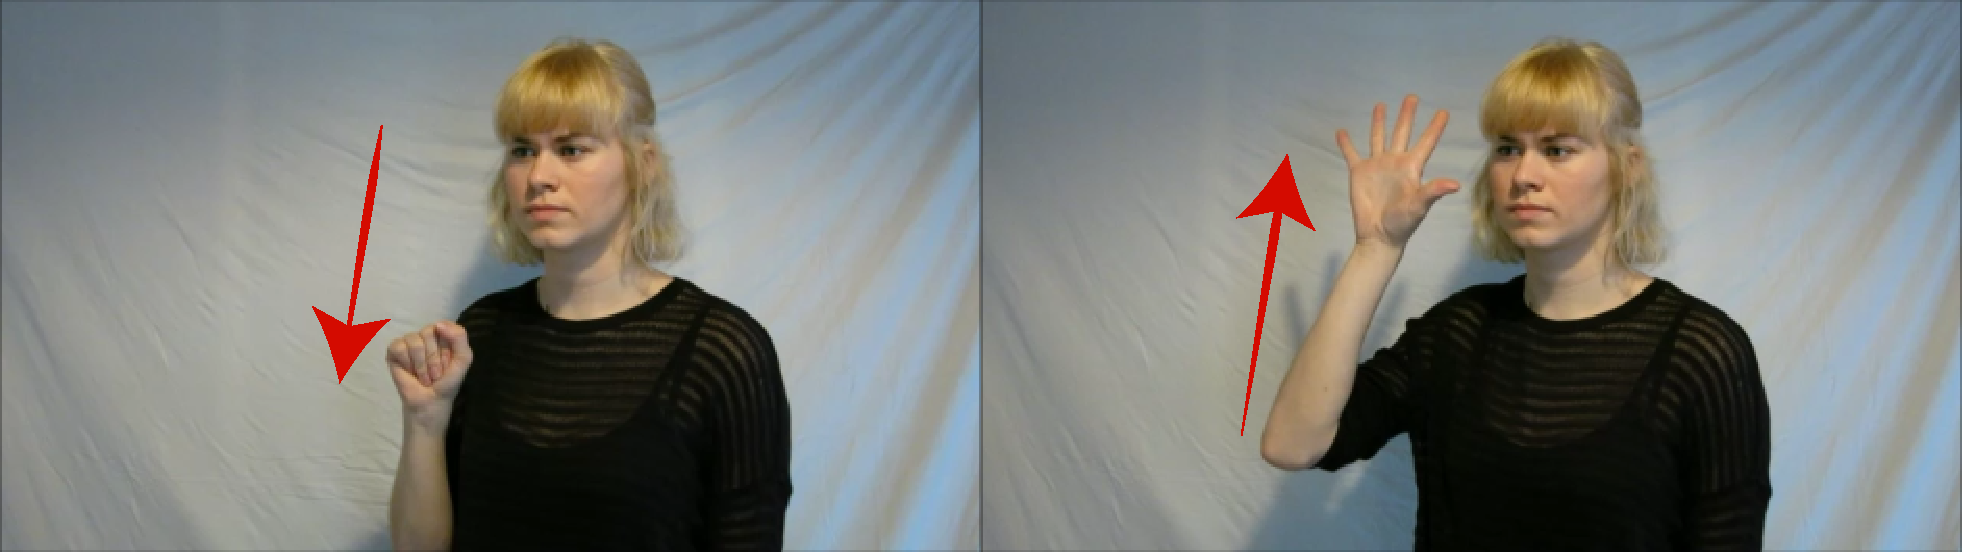
\includegraphics[resolution=300,width=0.9\textwidth]{Test1/Gestik-par/Gestik7_Pause}
	\caption{Illustration af gestik-par 7; hånden lukker sammen i den dynamisk, vertikal bevægelse nedad til pause og hånden åbner i den dynamisk, vertikal bevægelse opad til start.}
	\label{fig:GestikPar7Pause}
\end{figure}
\noindent
%


\section{Forslag til at skifte musiknummer}
\label{app:ForslagSkift}
%
Følgende fremgår de syv forskellige forslag til semaforiske gestikker, der kan knyttes til at skifte musiknummer.
%
\begin{figure}[H]
	\centering
	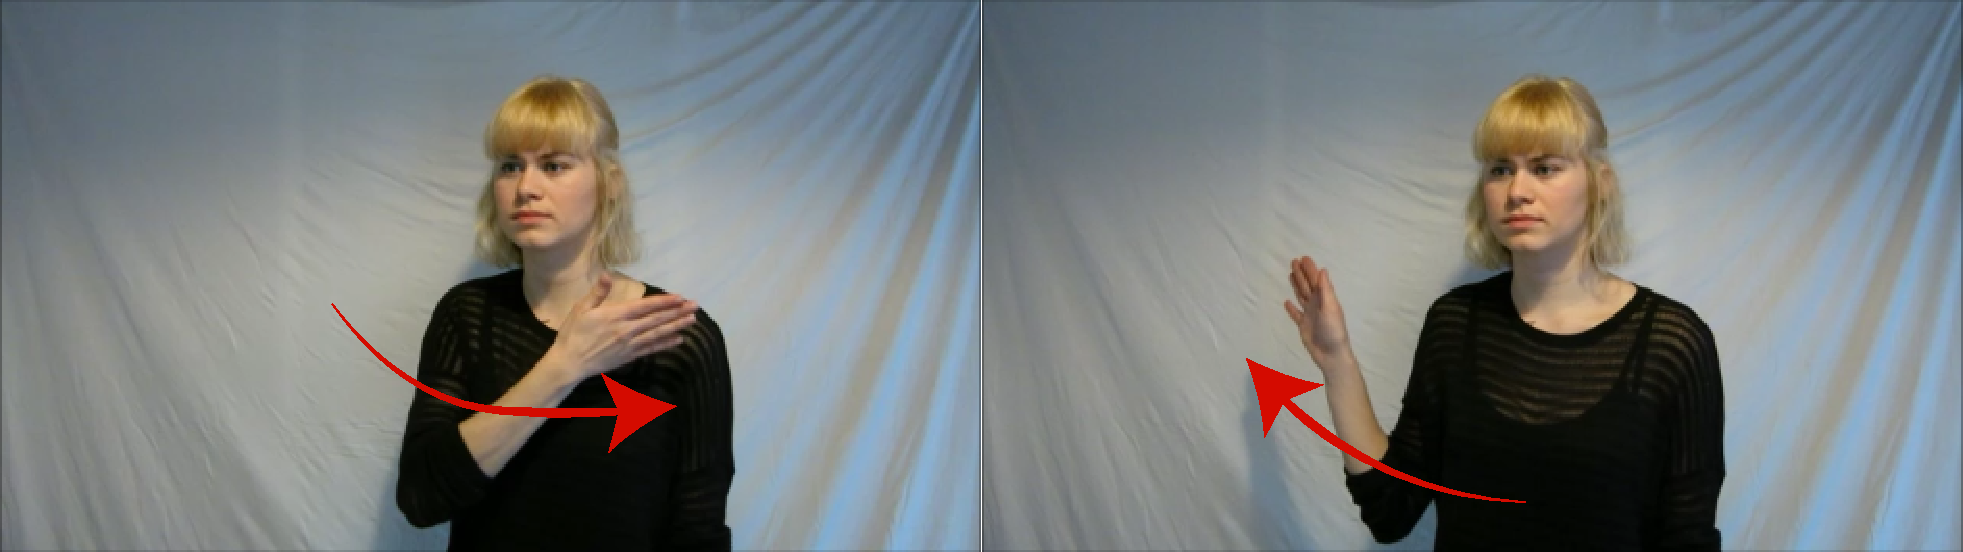
\includegraphics[resolution=300,width=0.9\textwidth]{Test1/Gestik-par/Gestik1_SkiftSang}
	\caption{Illustration af gestik-par 1; swipe fra højre mod venstre for at skifte til det næste musiknummer og fra venstre mod højre for at skifte til det forrige musiknummer.}
	\label{fig:GestikPar1SkiftApp}
\end{figure}
\noindent
%
%
\begin{figure}[H]
	\centering
	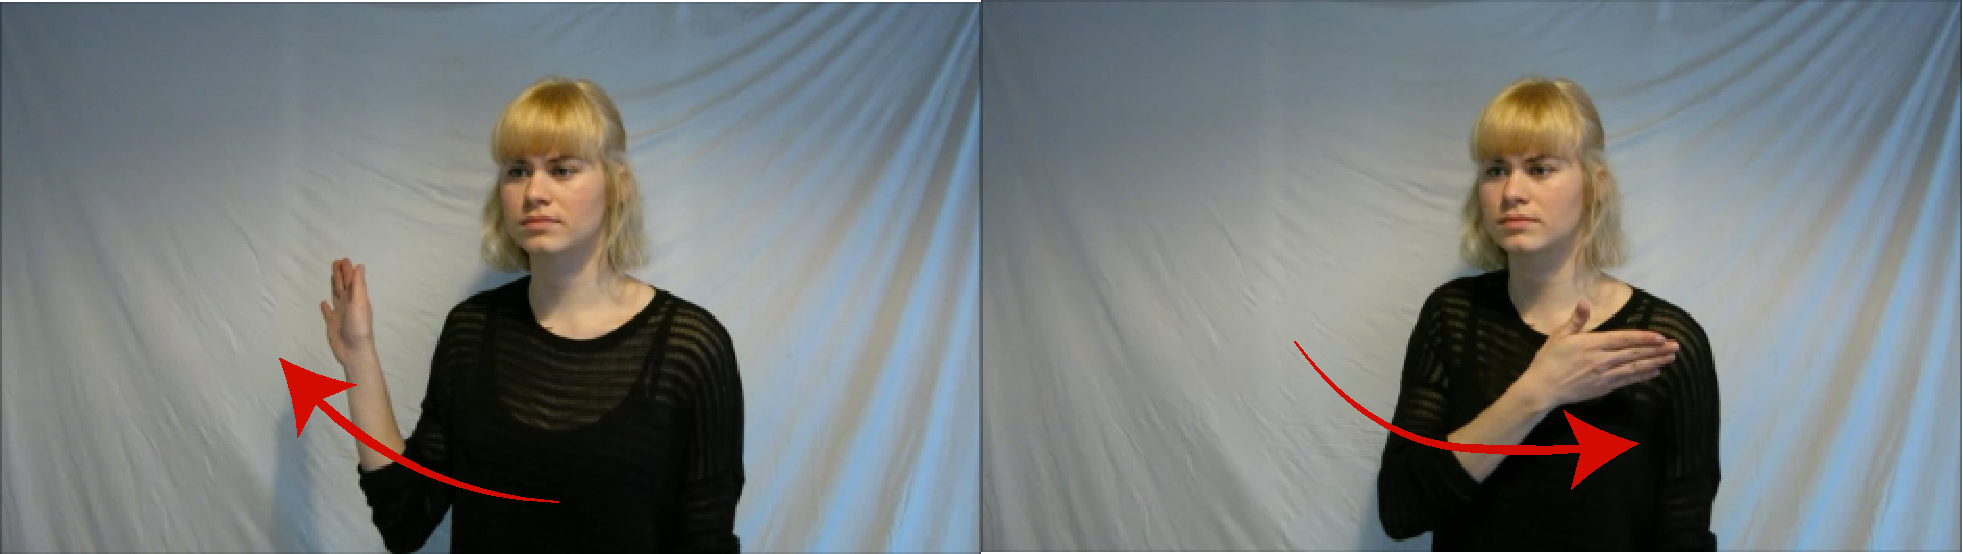
\includegraphics[resolution=300,width=0.9\textwidth]{Test1/Gestik-par/Gestik2_SkiftSang}
	\caption{Illustration af gestik-par 2; swipe fra venstre mod højre for at skifte til det næste musiknummer og fra højre mod venstre for at skifte til det forrige musiknummer.}
	\label{fig:GestikPar2SkiftApp}
\end{figure}
\noindent
%
%
\begin{figure}[H]
	\centering
	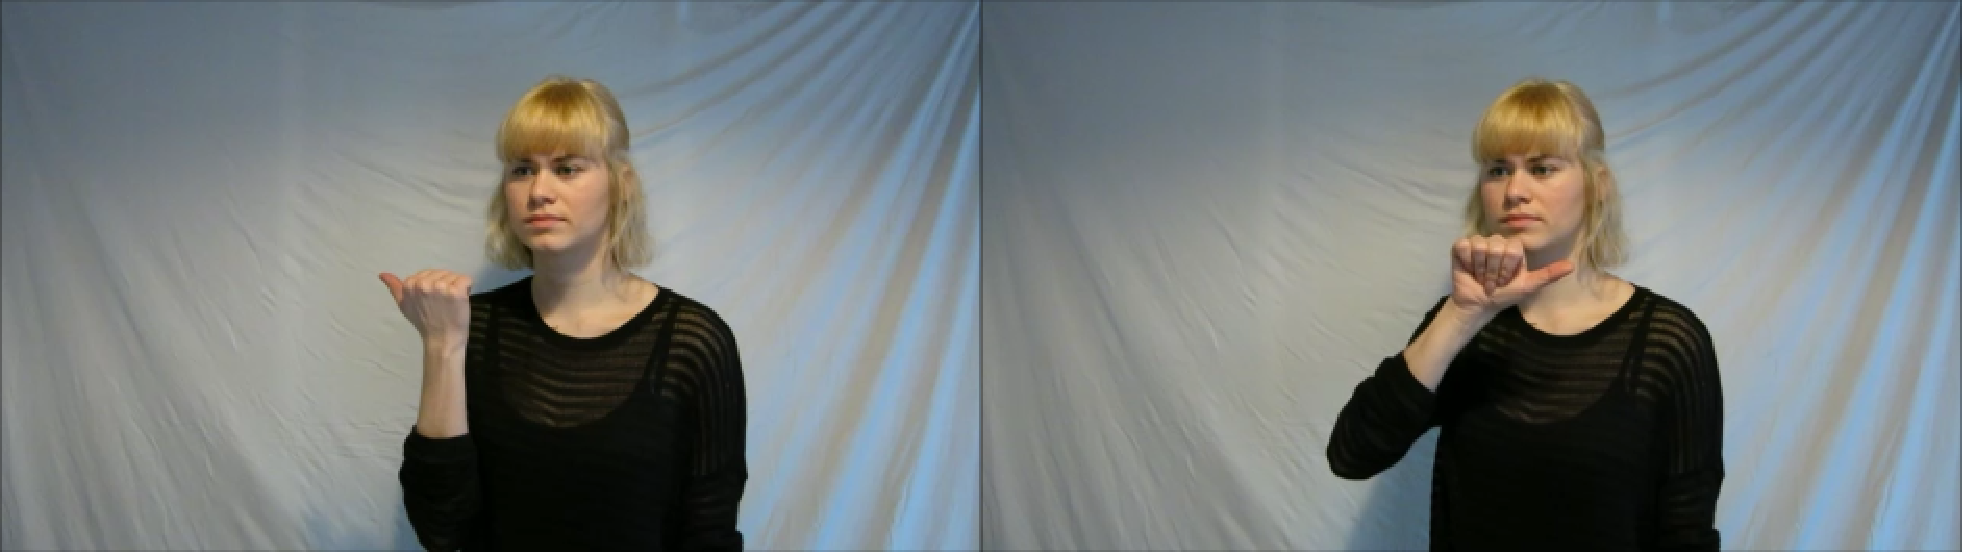
\includegraphics[resolution=300,width=0.9\textwidth]{Test1/Gestik-par/Gestik3_SkiftSang}
	\caption{Illustration af gestik-par 3; tommelfinger peger i den retning musiknummeret skal skifte i. Først frem og derefter til det forrige musiknummer.}
	\label{fig:GestikPar3SkiftApp}
\end{figure}
\noindent
%
%
\begin{figure}[H]
	\centering
	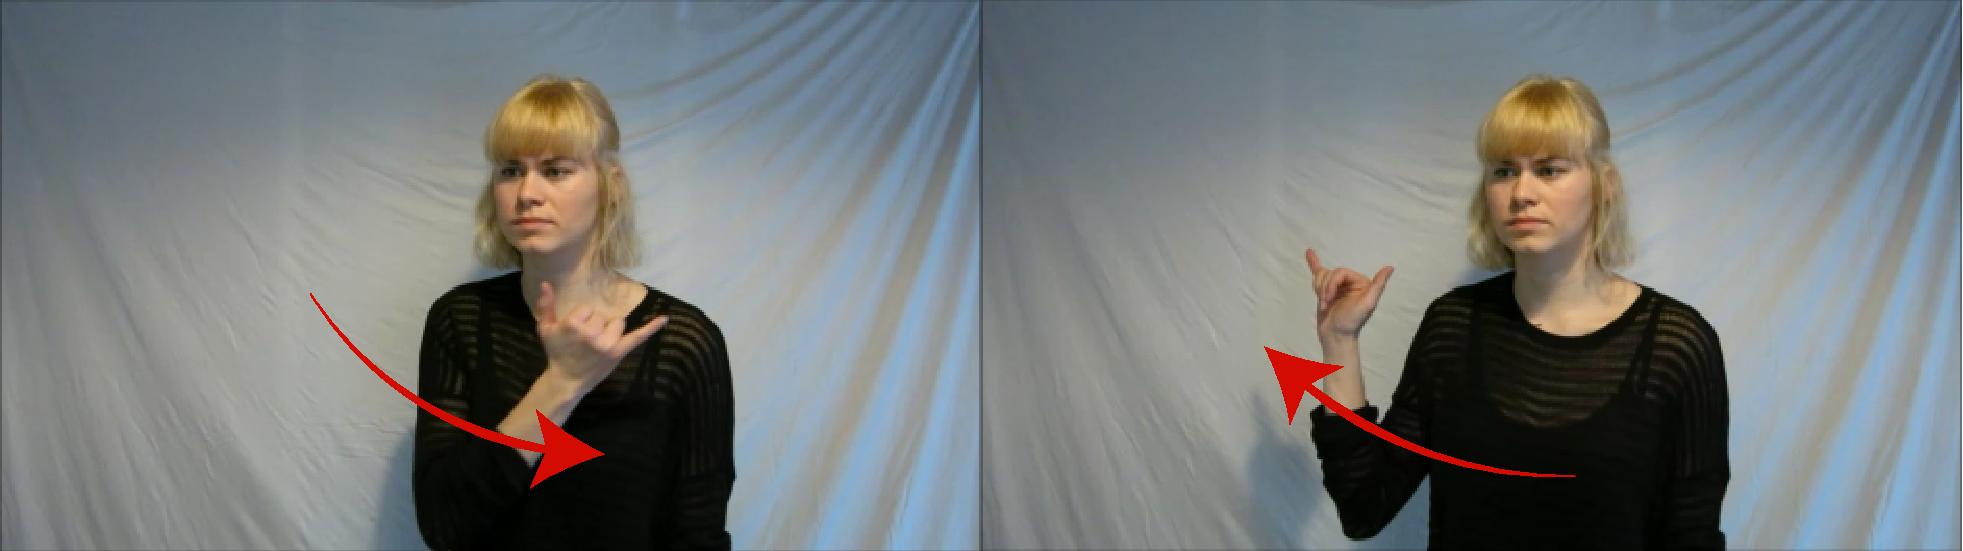
\includegraphics[resolution=300,width=0.9\textwidth]{Test1/Gestik-par/Gestik4_SkiftSang}
	\caption{Illustration af gestik-par 4; swipe fra højre mod venstre med tommel- og lillefinger strakt, mens de andre fingre bøjes for at skifte til det næste musiknummer og fra venstre mod højre for at skifte til det forrige musiknummer.}
	\label{fig:GestikPar4SkiftApp}
\end{figure}
\noindent
%
%
\begin{figure}[H]
	\centering
	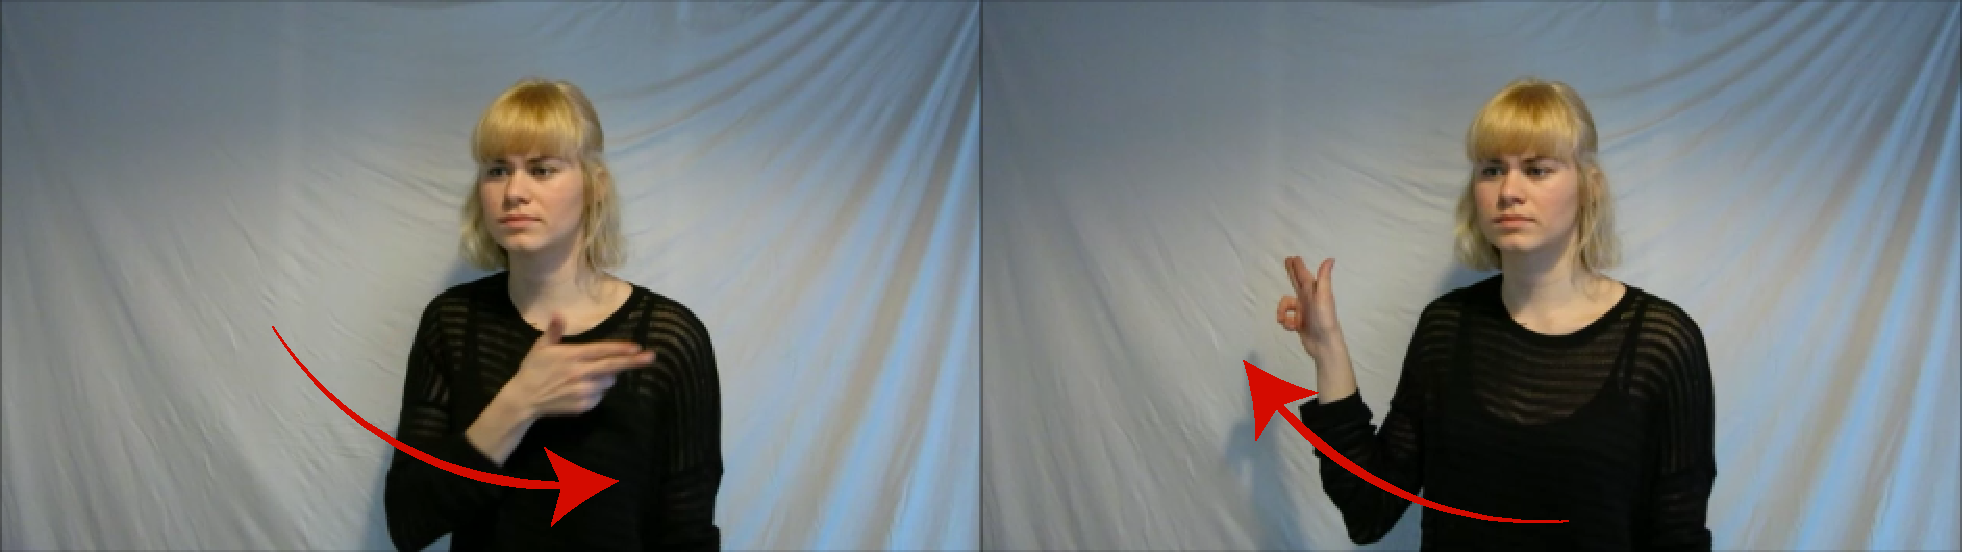
\includegraphics[resolution=300,width=0.9\textwidth]{Test1/Gestik-par/Gestik5_SkiftSang}
	\caption{Illustration af gestik-par 5; swipe med pege- og langefinger fra højre mod venstre for at skifte til det næste musiknummer og fra venstre mod højre for at skifte til det forrige musiknummer.}
	\label{fig:GestikPar5SkiftApp}
\end{figure}
\noindent
%
%
\begin{figure}[H]
	\centering
	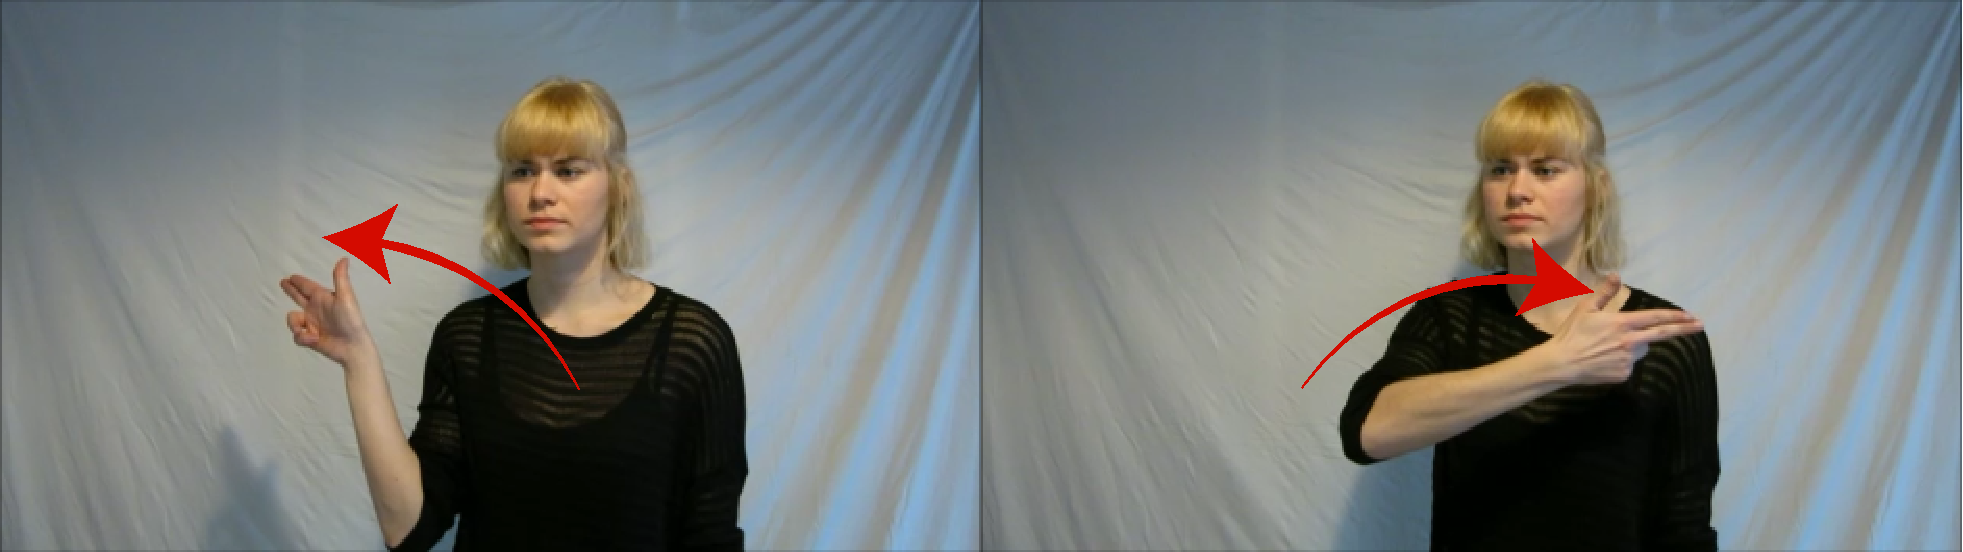
\includegraphics[resolution=300,width=0.9\textwidth]{Test1/Gestik-par/Gestik6_SkiftSang}
	\caption{Illustration af gestik-par 6; tommel-, pege- og langefinger holdes strakt mens de andre fingre bøjes samtidig med at hånden køres i en bue fra venstre mod højre og ender med at pege til højre for at skifte til det næste musiknummer og fra højre mod venstre for at skifte til det forrige musiknummer.}
	\label{fig:GestikPar6SkiftApp}
\end{figure}
\noindent
%
%
\begin{figure}[H]
	\centering
	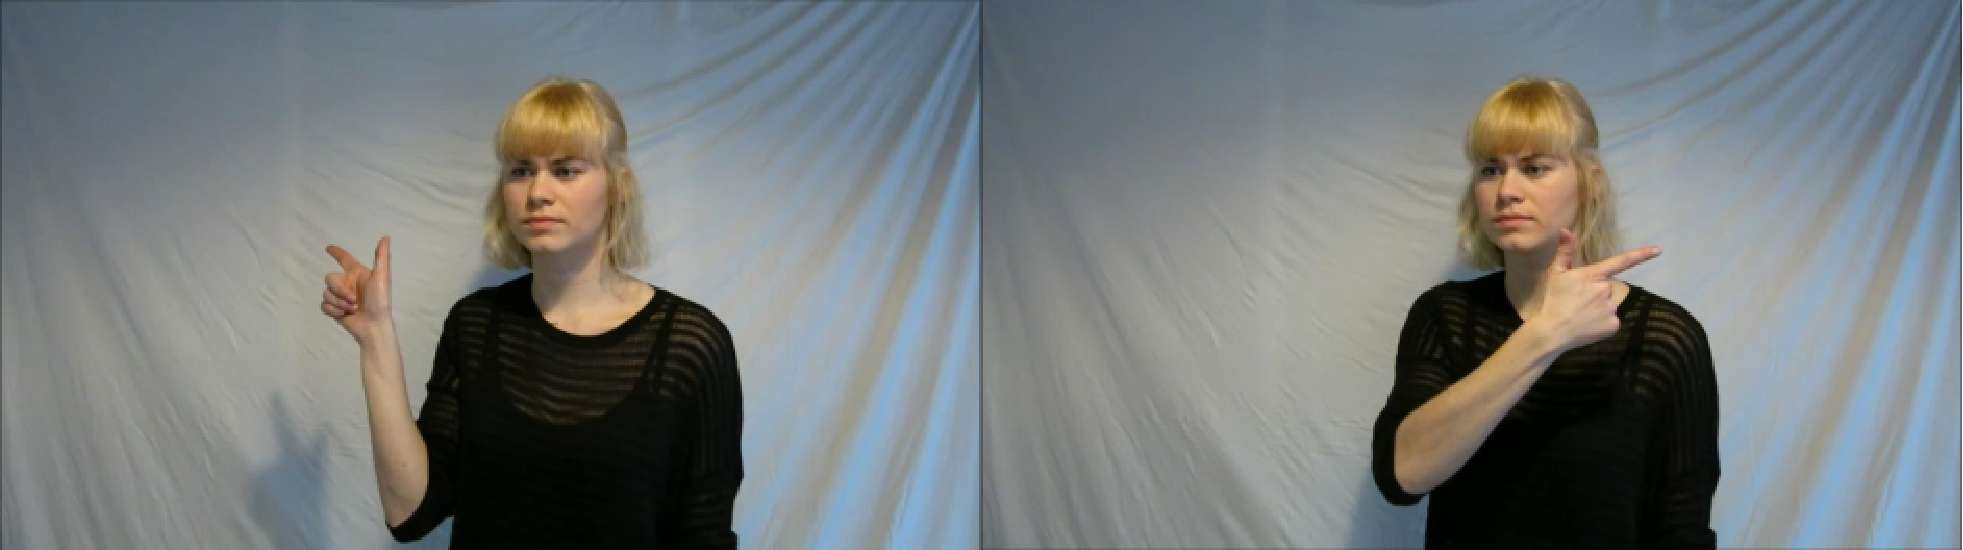
\includegraphics[resolution=300,width=0.9\textwidth]{Test1/Gestik-par/Gestik7_SkiftSang}
	\caption{Illustration af gestik-par 7; peg med tommel- og pegefinger strakt i den retning musiknummeret skal skifte i. Først frem og derefter til det forrige musiknummer.}
	\label{fig:GestikPar7SkiftApp}
\end{figure}
\noindent
%

\section{Forslag til justering af lydstyrken}
\label{app:ForslagVolumen}
%
Følgende fremgår de ni forskellige forslag til semaforiske gestikker, der kan knyttes til justere lydstyrken.
%
\begin{figure}[H]
	\centering
	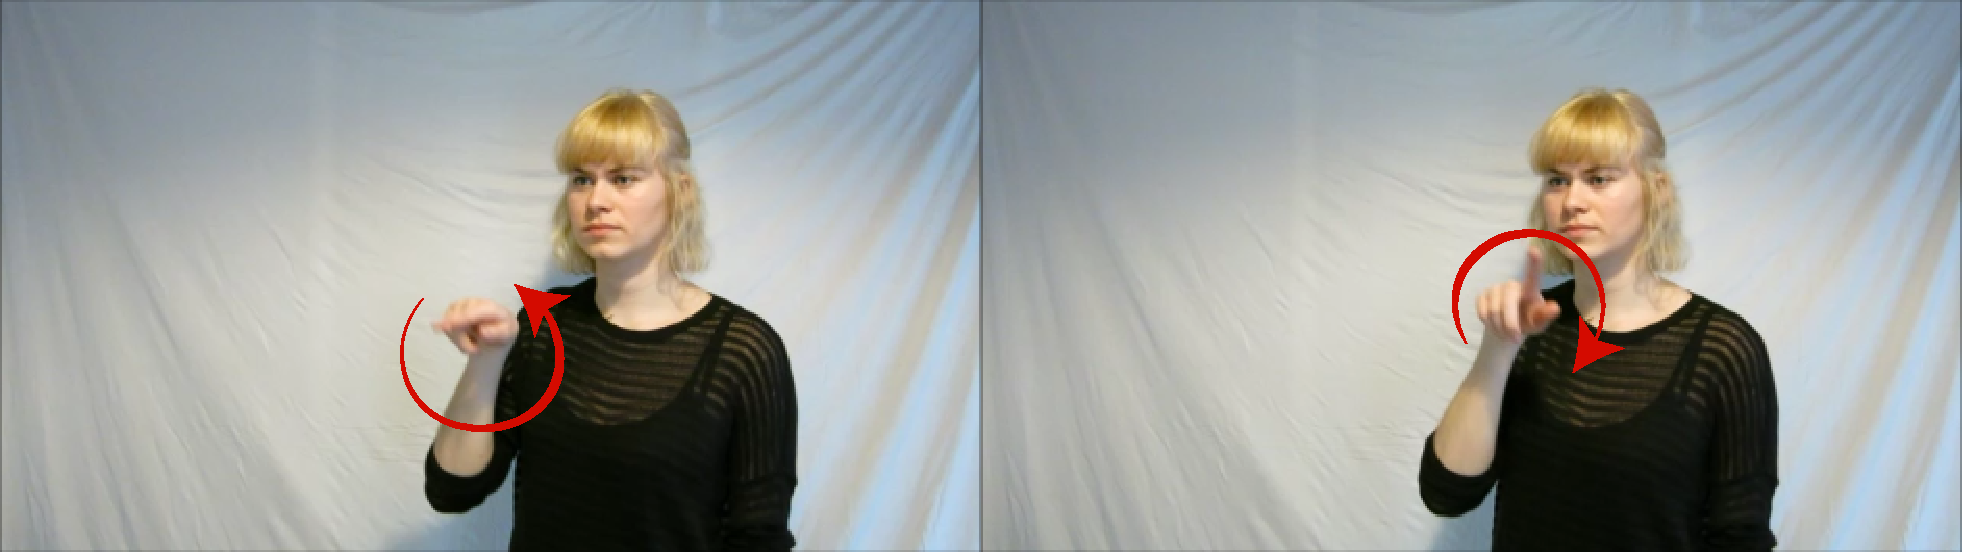
\includegraphics[resolution=300,width=0.9\textwidth]{Test1/Gestik-par/Gestik1_Volumen}
	\caption{Illustration af gestik-par 1; cirkulær bevægelse med pegefingeren i urets retning for at skrue op og mod uret for at skrue ned.}
	\label{fig:GestikPar1VolumenApp}
\end{figure}
\noindent
%
%
\begin{figure}[H]
	\centering
	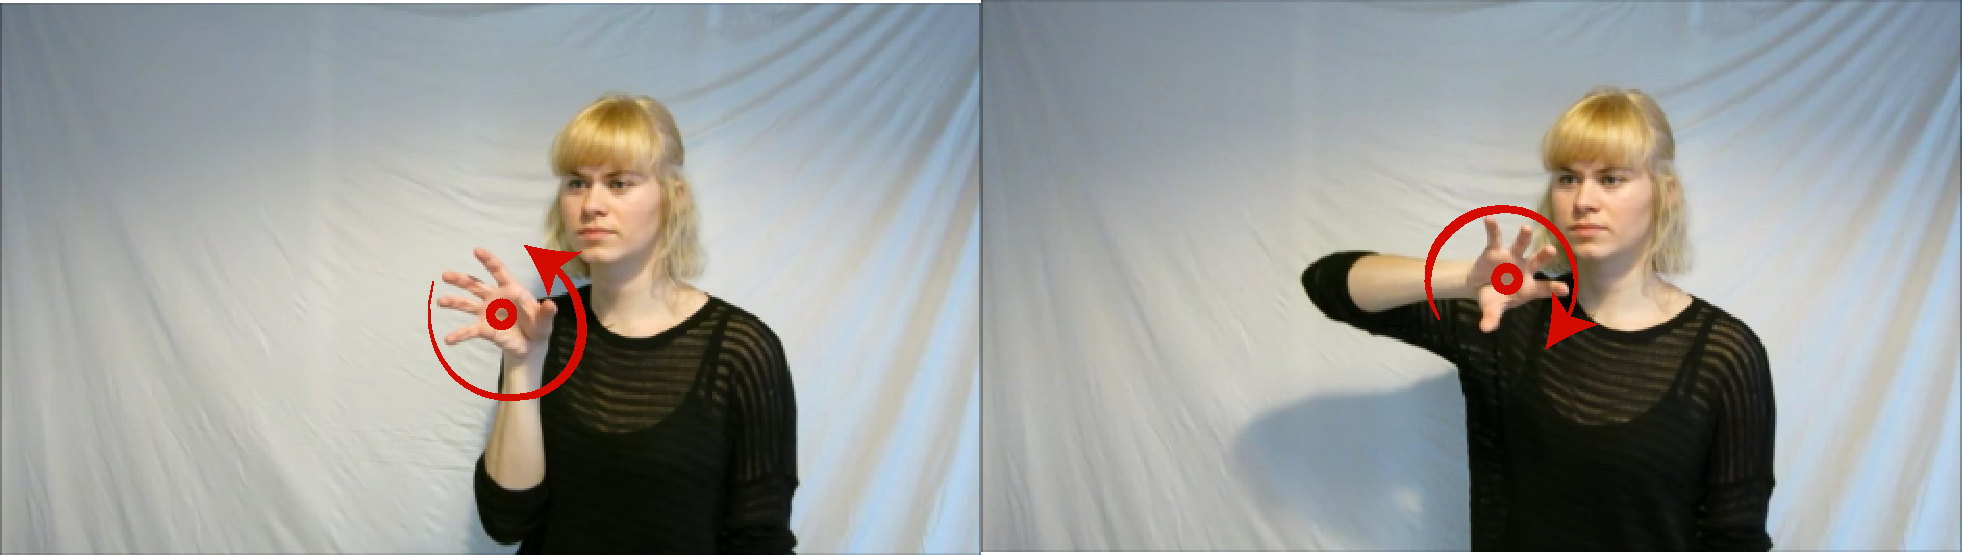
\includegraphics[resolution=300,width=0.9\textwidth]{Test1/Gestik-par/Gestik2_Volumen}
	\caption{Illustration af gestik-par 2; cirkulær bevægelse med halvbøjede fingre, ligesom hvis det var en drejeknap i urets retning for at skrue op og mod uret for at skrue ned.}
	\label{fig:GestikPar2VolumenApp}
\end{figure}
\noindent
%
%
\begin{figure}[H]
	\centering
	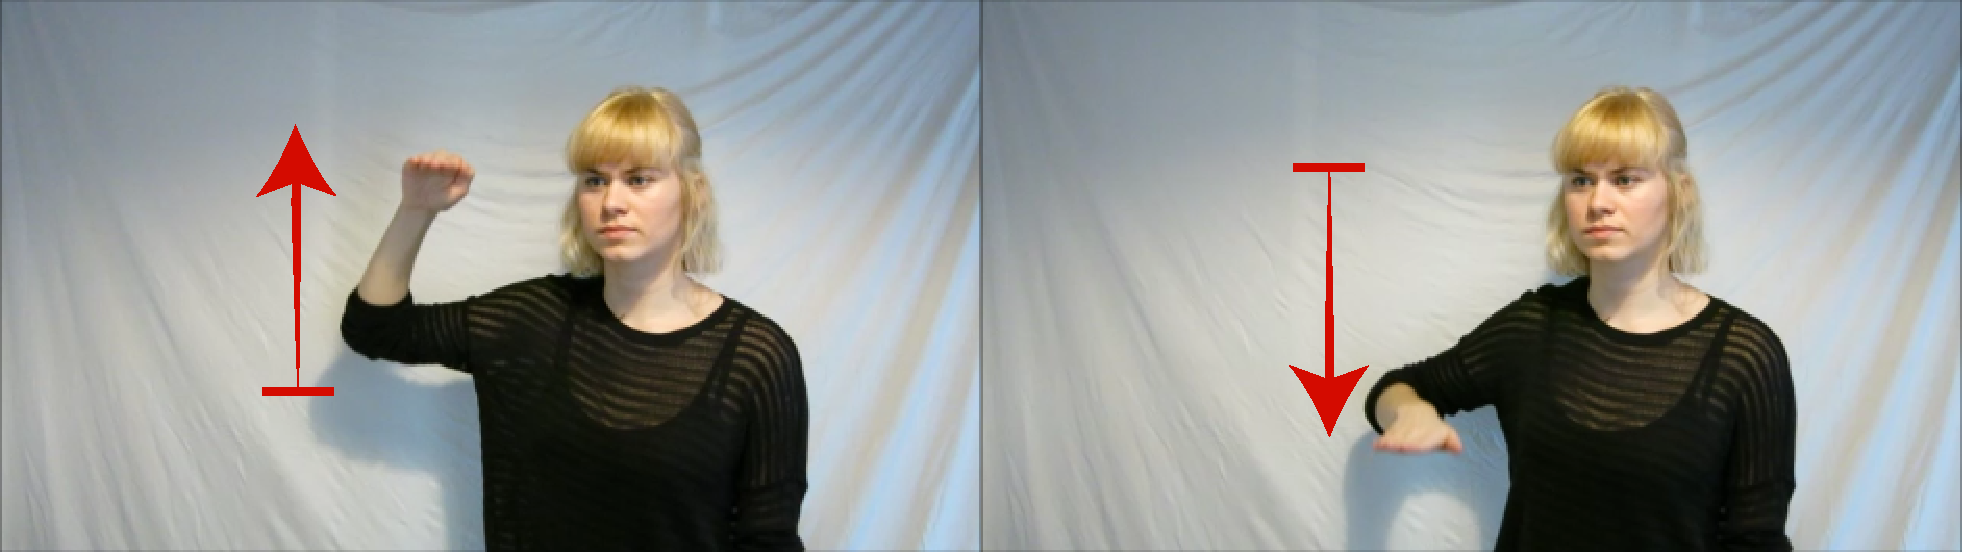
\includegraphics[resolution=300,width=0.9\textwidth]{Test1/Gestik-par/Gestik3_Volumen}
	\caption{Illustration af gestik-par 3; horisontal hånd løftes vertikalt med håndfladen nedad for at skrue op og for at skrue ned sænkes hånden vertikalt med håndfladen nedad.}
	\label{fig:GestikPar3VolumenApp}
\end{figure}
\noindent
%
%
\begin{figure}[H]
	\centering
	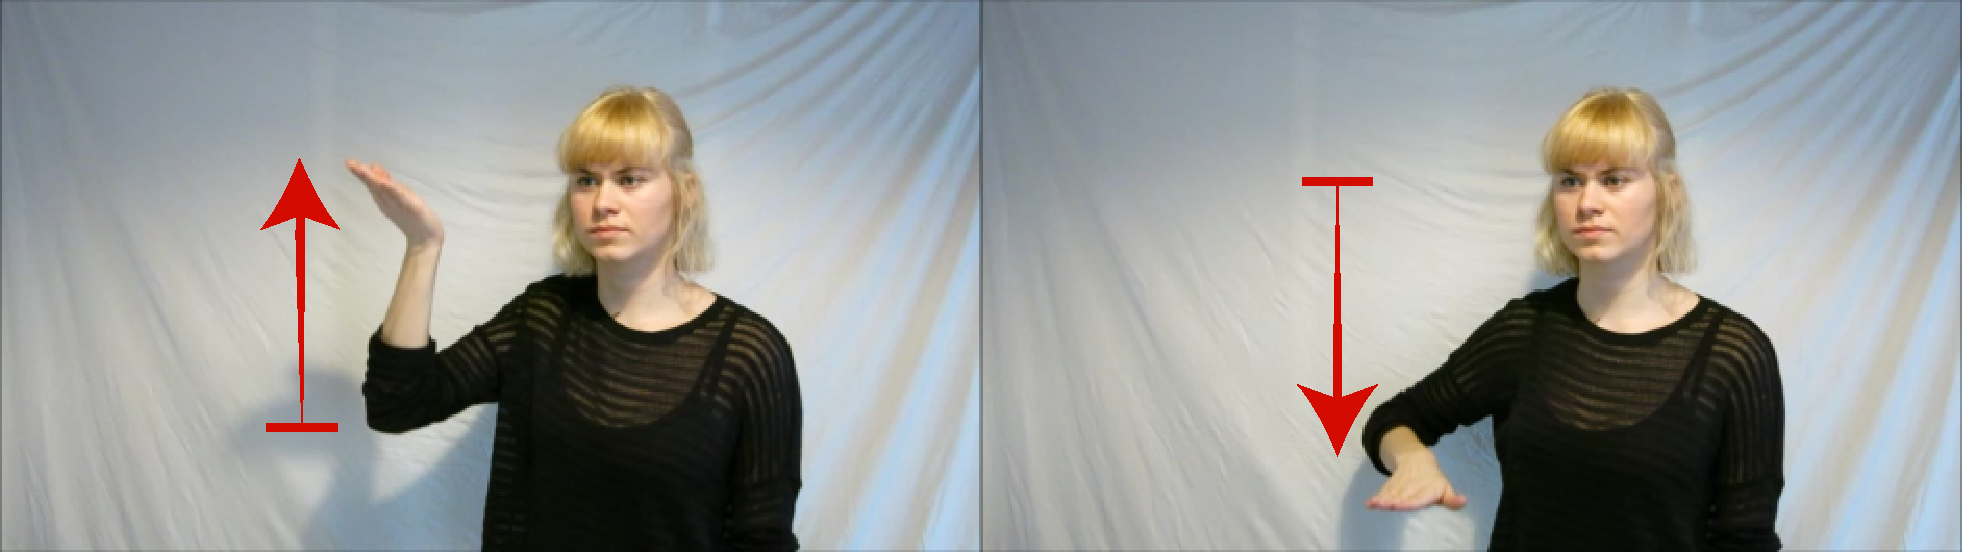
\includegraphics[resolution=300,width=0.9\textwidth]{Test1/Gestik-par/Gestik4_Volumen}
	\caption{Illustration af gestik-par 4; horisontal hånd løftes vertikalt med håndfladen opad for at skrue op og for at skrue ned sænkes hånden vertikalt med håndfladen nedad.}
	\label{fig:GestikPar4VolumenApp}
\end{figure}
\noindent
%
%
\begin{figure}[H]
	\centering
	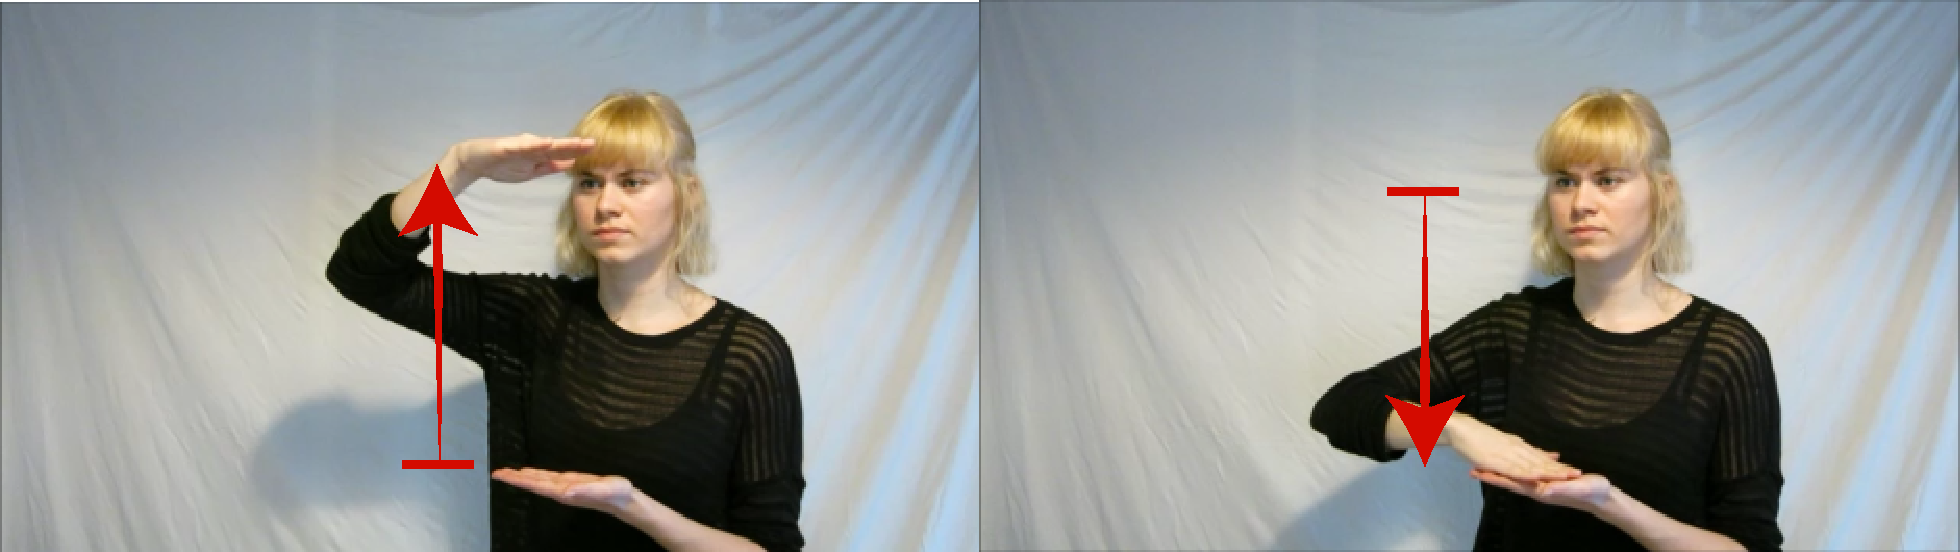
\includegraphics[resolution=300,width=0.9\textwidth]{Test1/Gestik-par/Gestik5_Volumen}
	\caption{Illustration af gestik-par 5; horisontal ikke-dominant hånd med håndfladen opad holdes stationær, mens den dominante hånd ligeledes holde horisontal med håndfladen nedad men løftes vertikalt væk fra den ikke-dominante hånd for at skrue op og sænkes mod den ikke-dominante hånd for at skrue ned.}
	\label{fig:GestikPar5VolumenApp}
\end{figure}
\noindent
%
%
\begin{figure}[H]
	\centering
	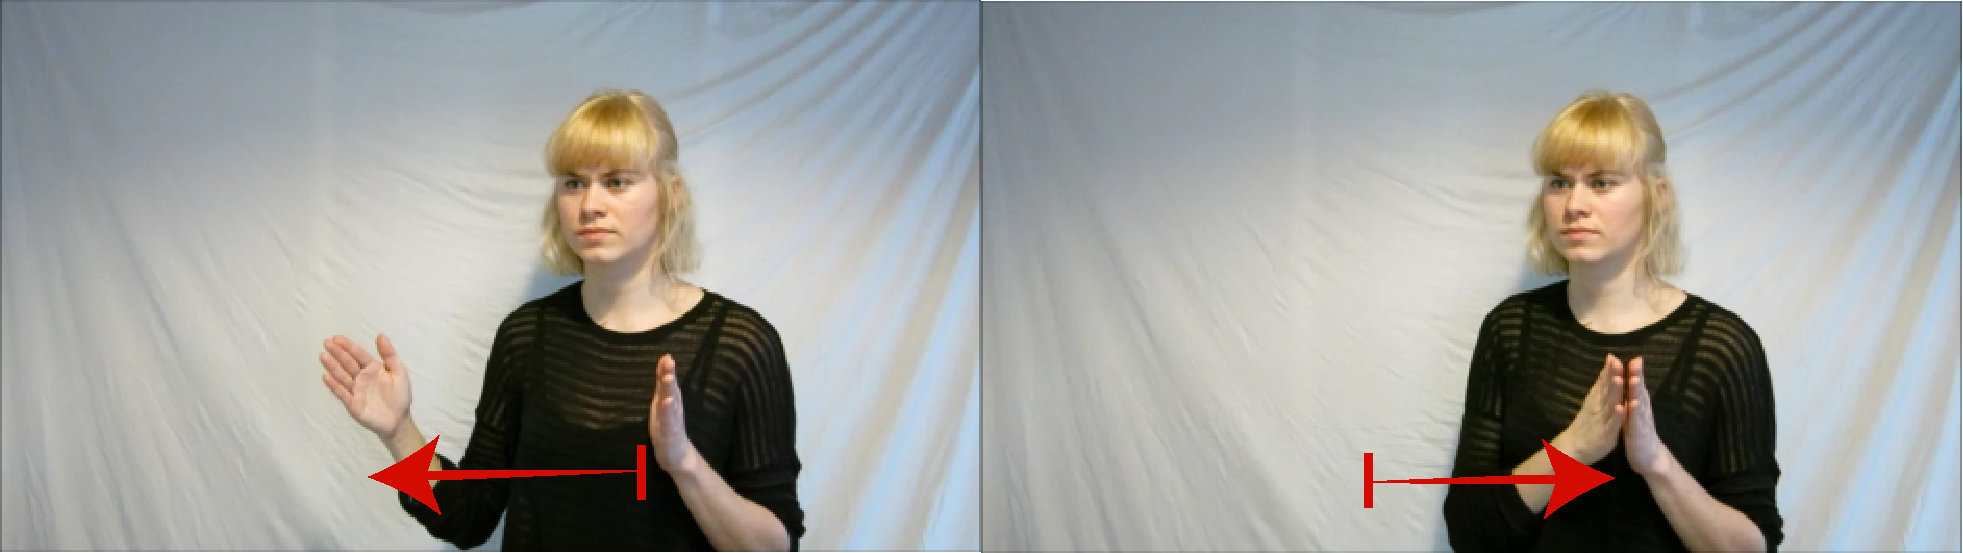
\includegraphics[resolution=300,width=0.9\textwidth]{Test1/Gestik-par/Gestik6_Volumen}
	\caption{Illustration af gestik-par 6; vertikal ikke-dominant hånd holdes stationær, ems den dominante hånd ligeledes holdes vertikal og bevægelser sig væk fra den ikke-dominante hånd i en horisontal bevægelse for at skrue op og for at skrue ned bevæges den dominante hånd mod den ikke-dominante hånd.}
	\label{fig:GestikPar6VolumenApp}
\end{figure}
\noindent
%
%
\begin{figure}[H]
	\centering
	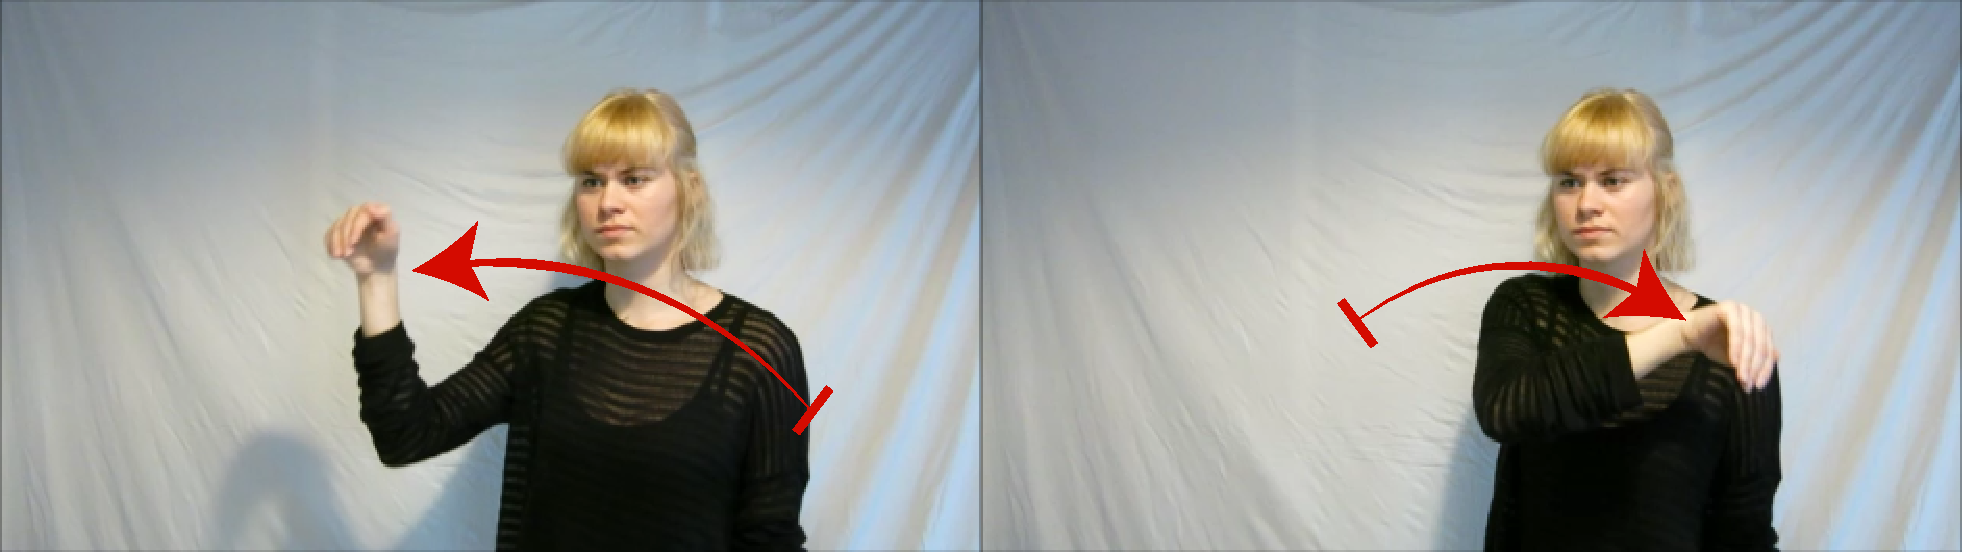
\includegraphics[resolution=300,width=0.9\textwidth]{Test1/Gestik-par/Gestik7_Volumen}
	\caption{Illustration af gestik-par 7; krum hånd bevæges i en bue fra venstre mod højre for at skrue op og fra højre mod venstre for at skrue ned svarende til hvordan det gøres på A9, \parencite{WEB:BeoplayA9}.}
	\label{fig:GestikPar7VolumenApp}
\end{figure}
\noindent
%
%
\begin{figure}[H]
	\centering
	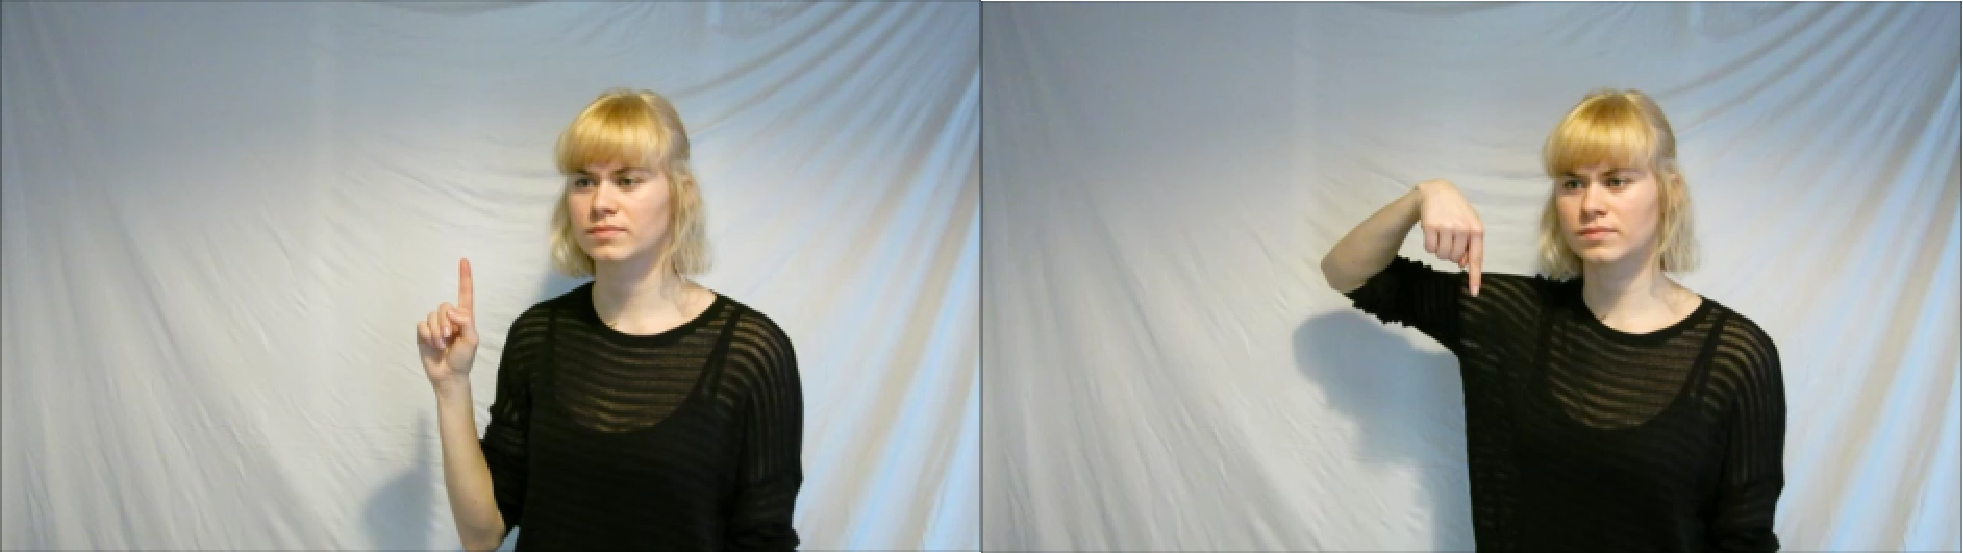
\includegraphics[resolution=300,width=0.9\textwidth]{Test1/Gestik-par/Gestik8_Volumen}
	\caption{Illustration af gestik-par 8; pegefingeren peger op for at skrue op og peger ned for at skrue ned.}
	\label{fig:GestikPar8VolumenApp}
\end{figure}
\noindent
%
%
\begin{figure}[H]
	\centering
	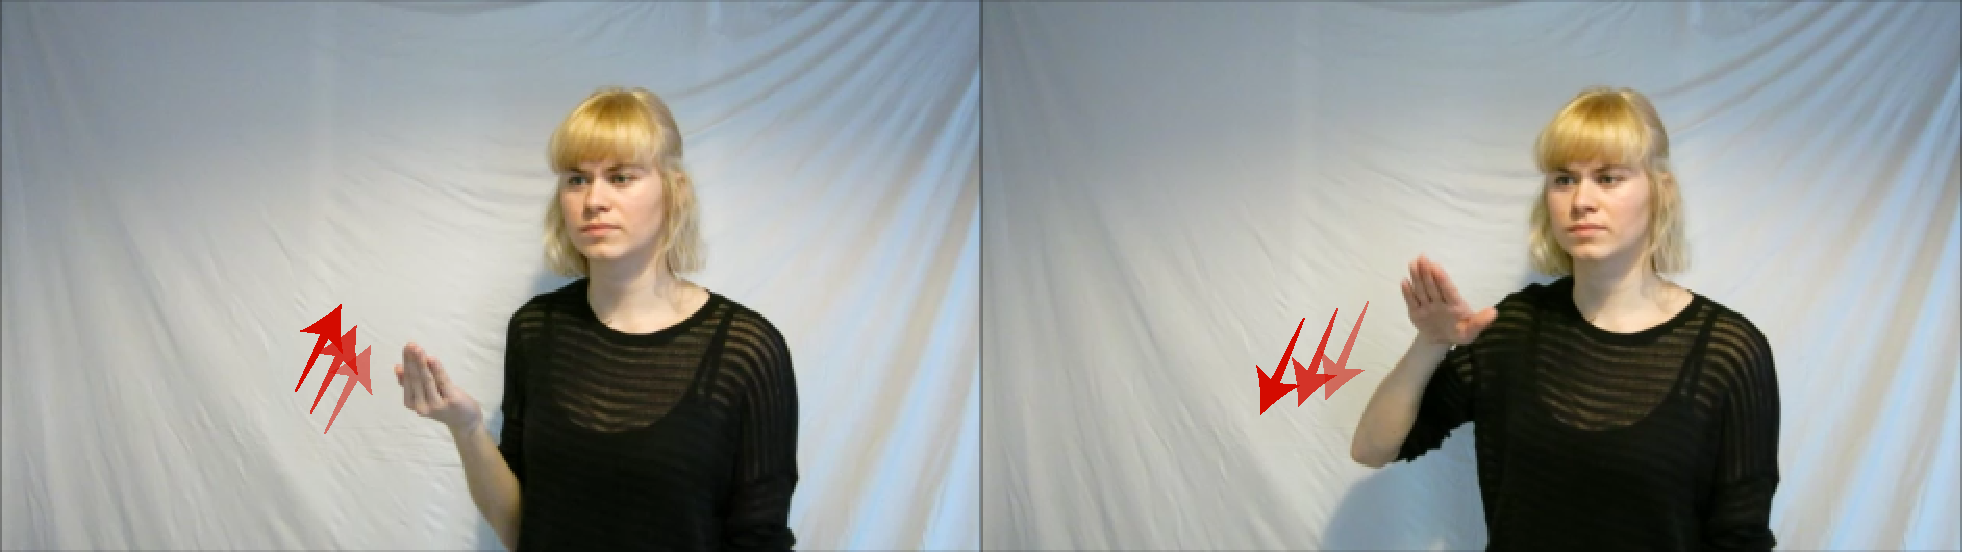
\includegraphics[resolution=300,width=0.9\textwidth]{Test1/Gestik-par/Gestik9_Volumen}
	\caption{Illustration af gestik-par 9; \enquote{kom så}-bevægelse med fingrene for at skrue op og \enquote{ro på}-bevægelse med fingrene for at skrue ned.}
	\label{fig:GestikPar9VolumenApp}
\end{figure}
\noindent
%